\documentclass[aspectratio=169]{beamer}
\mode<presentation>{
\usetheme{default}
}

\usepackage{graphicx} 
\usepackage{booktabs} 
\usepackage{graphicx,color}
\usepackage{minted} %extrai python com sitaxe destacada
\usepackage{pgfplots}
\usepackage{tikz}

\title[Short title]{Theano} 
\subtitle{Intel-Unesp/NCC - Machine Learning and High Performance Computing Team}
\author{Machine Learning Team}

\begin{document}
\begin{frame}
\titlepage 
\end{frame}

\begin{frame}
\frametitle{Overview} 
\begin{itemize}
\item Introduction to Theano
\item What is Theano? Is it a programming language?
\item Basic Algebra
\item Logistic Function in Theano - A Neural Activation Function
\item Functions with Multiple Output
\item Theano: Using Shared Variables
\item Theano: Computing Gradiates
\item Theano: Math Challenge
\item References
\end{itemize}
\end{frame}

%-S1
\begin{frame}
\frametitle{Introduction to Theano}
Theano is a Python library that lets you to define, optimize, and evaluate mathematical expressions.
\\[1.0cm]
Theano combines aspects of a computer algebra system (CAS) with aspects of an optimizing compiler. 
\end{frame}
%-S1

%-S2
\begin{frame}
\frametitle{Introduction to Theano}
\emph{Symbolic Expression}
\\[0.5cm]
Creating the tensors
\inputminted{python}{./aux_files/t1.py}
\end{frame}
%-S2

%-S3
\begin{frame}
\frametitle{Introduction to Theano}
Design an expression with the tensors
\inputminted{python}{./aux_files/t2.py}
\end{frame}
%-S3

%-S4
\begin{frame}
\frametitle{Introduction to Theano}
Transforming the expression in a callable code
\inputminted{python}{./aux_files/t3.py}
\end{frame}
%-S4

%-S5
\begin{frame}
\frametitle{Introduction to Theano}
Calling the object code (evaluating the function with real parameters)
\inputminted{python}{./aux_files/t4.py}
\end{frame}
%-S5

%-S6
\begin{frame}
\frametitle{Theano: Is it a programming language?}
When programming in theano you have to:
\begin{enumerate}
\item  declare variables and to define their types
\item  build expressions for how to put those variables together
\item  compile expression graphs to functions in order to use them for computation.
\end{enumerate}
So, what is Theano?
\end{frame}
%-S6

%-S7
\begin{frame}
\frametitle{Theano: Is it a programming language?}
\emph{It is good to think of theano as the interface to a compiler which can build a callable object from a purely symbolic graph. 
\\[1.0cm]
One of Theano’s most important features is that theano.function can optimize a graph and compile some or all of it into native machine instructions. }
\end{frame}
%-S7

%-S8
\begin{frame}
\frametitle{Theano: Basic Algebra}
Adding two matrices:
\inputminted{python}{./aux_files/t5.py}
\end{frame}
%-S8

%S9
\begin{frame}
\frametitle{Theano: Basic Algebra. \textit{HandsOn!} }
Exercise: Run this fragment. What is/are the result(s)?  
\\[0.5cm]
\inputminted{python}{./aux_files/t6.py}
\end{frame}
%-S9

%-S10
\begin{frame}
\frametitle{Theano: \textit{Logistic Function} }
Let's compute the Logistic Curve
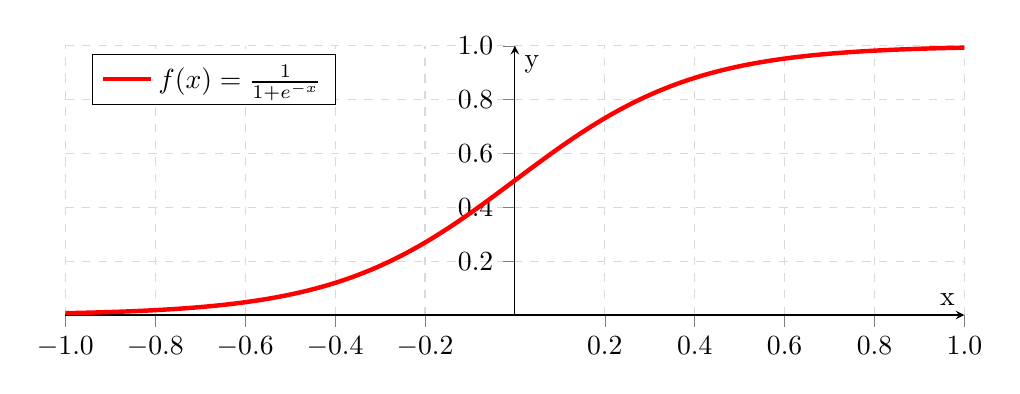
\begin{tikzpicture}
    \begin{axis}[
        legend pos=north west,
        axis x line=middle,
        axis y line=middle,
        x tick label style={/pgf/number format/fixed,
                            /pgf/number format/fixed zerofill,
                            /pgf/number format/precision=1},
        y tick label style={/pgf/number format/fixed,
                            /pgf/number format/fixed zerofill,
                            /pgf/number format/precision=1},
        grid = major,
        width=13cm,
        height=5cm,
        grid style={dashed, gray!30},
        xmin=-1,     % start the diagram at this x-coordinate
        xmax= 1,    % end   the diagram at this x-coordinate
        ymin= 0,     % start the diagram at this y-coordinate
        ymax= 1,   % end   the diagram at this y-coordinate
        %axis background/.style={fill=white},
        xlabel=x,
        ylabel=y,
        tick align=outside,
        enlargelimits=false]
        % plot the stirling-formulae
        \addplot[domain=-1:1, red, ultra thick,samples=500] {1/(1+exp(-5*x))};
        \addlegendentry{$f(x)=\frac{1}{1+e^{-x}}$}
    \end{axis}
\end{tikzpicture}
\end{frame}
%-S10

%-S11
\begin{frame}
\frametitle{Theano Code: \emph{Logistic Function} }
\inputminted{python}{./aux_files/t7.py}
\end{frame}
%-S11

%-S12
\begin{frame}
\frametitle{Theano: Functions with Multiple Output}
\inputminted{python}{./aux_files/t8.py}
\end{frame}
%-S12

%-S13
\begin{frame}
\frametitle{Theano: Using Shared Variables}
It is possible to build functions that memorize their internal states. In this case, at the beginning, the state is  zero.Then, on each function call, the state is incremented by the function’s argument.
\inputminted{python}{./aux_files/t9.py}
\end{frame}
%-S13

%-S14
\begin{frame}
\frametitle{Theano: Computing Gradients }
Let's create a function to compute the derivative of some expression  \textit{y} with respect to its parameter \textit{x}.
$y(x) = x^{2}$
\inputminted{python}{./aux_files/t10.py}
\end{frame}
%-S14

\begin{frame}
\frametitle{References}
\footnotesize{
\begin{thebibliography}{99}
\bibitem[Theano - Online Theano Documentation]{p1} Theano  Documentation - http://deeplearning.net/software/theano/
\bibitem[Python Deep Learning]{p2} ZOCCA, V.; \textit{et.al.} Python Deep Learning. London:Packt Books, 2017


\end{thebibliography}
}
\end{frame}


\end{document}
